%% 2/18/2016
%%%%%%%%%%%%%%%%%%%%%%%%%%%%%%%%%%%%%%%%%%%%%%%%%%%%%%%%%%%%%%%%%%%%%%%%%%%%
% AGUJournalSample.tex: this sample file is for articles formatted with LaTeX
%
% This sample file includes commands and instructions
% given in the order necessary to produce a final output that will
% satisfy AGU requirements.
%
% PLEASE DO NOT USE YOUR OWN MACROS
% DO NOT USE \newcommand, \renewcommand, or \def.
%
% FOR FIGURES, DO NOT USE \psfrag or \subfigure.
% DO NOT USE \psfrag or \subfigure commands.
%
%%%%%%%%%%%%%%%%%%%%%%%%%%%%%%%%%%%%%%%%%%%%%%%%%%%%%%%%%%%%%%%%%%%%%%%%%%%%
%
% Step 1: Set the \documentclass
%
% There are two options for article format:
%
% 1) PLEASE USE THE DRAFT OPTION TO SUBMIT YOUR PAPERS.
% The draft option produces double spaced output.
%
% 2) numberline will give you line numbers.

% Tip:
%  To add line numbers to lines in equations:
%  \begin{linenomath*}
%  \begin{equation}
%  \end{equation}
%  \end{linenomath*}

%% To submit your paper:
\documentclass[linenumbers,draft]{agujournal}

% Now, type in the journal name: \journalname{<Journal Name>}
% ie,
\journalname{JGR-Earth Surface}

%% Choose from this list of Journals:
%
% JGR-Atmospheres
% JGR-Biogeosciences
% JGR-Earth Surface
% JGR-Oceans
% JGR-Planets
% JGR-Solid Earth
% JGR-Space Physics
% Global Biochemical Cycles
% Geophysical Research Letters
% Paleoceanography
% Radio Science
% Reviews of Geophysics
% Tectonics
% Space Weather
% Water Resource Research
% Geochemistry, Geophysics, Geosystems
% Journal of Advances in Modeling Earth Systems (JAMES)
% Earth's Future
% Earth and Space Science


%% ------------------------------------------------------------------------ %%
%
%  ENTER Title Page commands:
%
%% ------------------------------------------------------------------------ %%

% (A title should be specific, informative, and brief. Use
% abbreviations only if they are defined in the abstract. Titles that
% start with general terms then specific results are optimized in
% searches)

% Example: \title{This is a test title}

% (List authors by first name or initial followed by last name and
% separated by commas. Use \affil{} to number affiliations, and
% \thanks{} for author notes.
% Additional author notes should be indicated with \thanks{} (for
% example, for current addresses).

% Example: \authors{A. B. Author\affil{1}\thanks{Current address, Antartica}, B. C. Author\affil{2,3}, and D. E.
% Author\affil{3,4}\thanks{Also funded by Monsanto.}}

% (include name and email addresses of the corresponding author.  More
% than one corresponding author is allowed in this LaTeX file and for
% publication; but only one corresponding author is allowed in our
% editorial system.)

%% Corresponding Author:
% Corresponding author mailing address and e-mail address:

% Example: \correspondingauthor{First and Last Name}{email@address.edu}

% Authors are individuals who have significantly contributed to the
% research and preparation of the article. Group authors are allowed, if
% each author in the group is separately identified in an appendix.)

% \affiliation{1}{First Affiliation}
% \affiliation{2}{Second Affiliation}
% \affiliation{3}{Third Affiliation}
% \affiliation{4}{Fourth Affiliation}

%% Keypoints, final entry on title page.
% Example:
% \begin{keypoints}
% \item	List up to three key points (at least one is required)
% \item	Key Points summarize the main points and conclusions of the article
% \item	Each must be 100 characters or less with no special
% characters or punctuation
% \end{keypoints}

%% \begin{abstract} begins second page

%%%%%%%%%%%%%%%%%%%%%%%%%%%%%%%%%%%%%%%%%%%%%%%%%%%%%%%%%%%%%%%%%%%%%
% Track Changes:
% To add words, \added{<word added>}
% To delete words, \deleted{<word deleted>}
% To replace words, \replaced{<word to be replaced>}{<replacement word>}
% To explain why change was made: \explain{<explanation>}

% At the end of the document, use \listofchanges, which will list the
% changes and the page and line number where the change was made.

% When final version, \listofchanges will not produce anything,
% \added{} word will be printed, \deleted{} will take away the word,
% \replaced{}{} will print only the 2nd argument.
% \explain will not print anything.

% Optional argument:
% You can also add additional information to be printed with the list
% of changes, to indicate the initials of the person changing the text,
% and the time and/or date of the change, or any other comment by using
% the optional [] argument:
% \added[AH, 3:30pm, Feb 18, 2016]{added term}
% will yield
% [AH, 3:30pm, Feb 18, 2016] added term on page...
%%%%%%%%%%%%%%%%%%%%%%%%%%%%%%%%%%%%%%%%%%%%%%%%%%%%%%%%%%%%%%%%%%%%%

\begin{document}

%% ------------------------------------------------------------------------ %%
%
%  TITLE
%
%% ------------------------------------------------------------------------ %%


\title{Modeling the Shape and Evolution of Normal-Fault Facets}


%% ------------------------------------------------------------------------ %%
%
%  AUTHORS AND AFFILIATIONS
%
%% ------------------------------------------------------------------------ %%

 \authors{Gregory E.\ Tucker\affil{1}\thanks{Current address, McMurdo Station,
 Antartica},
 Frog2\affil{1,2}, Frog3\affil{3}}

\affiliation{1}{Cooperative Institute for Research in Environmental Sciences and Department of Geological Sciences,
University of Colorado, Boulder, Colorado, USA.}
\affiliation{2}{Frog Pond.}
\affiliation{3}{Toad Pond.}


%% Corresponding Author
%(include name and email addresses of the corresponding author.  More
%than one corresponding author is allowed in this Word file and for
%publication; but only one corresponding author is allowed in our
%editorial system.)

\correspondingauthor{A. B. Smith}{email@address.edu}

%  List up to three key points (at least one is required)
%  Key Points summarize the main points and conclusions of the article
%  Each must be 100 characters or less with no special characters or punctuation

\begin{keypoints}
\item Evolution of raw ensemble forecast \replaced{skill}{skills}
\item Future benefits from statistical post-processing
\item Global distribution of forecast skill development
\end{keypoints}

%% ------------------------------------------------------------------------ %%
%
%  ABSTRACT
%
%% ------------------------------------------------------------------------ %%


\begin{abstract}
this is a highly abstract paper
\end{abstract}

%% ------------------------------------------------------------------------ %%
%
%  TEXT
%
%% ------------------------------------------------------------------------ %%

%%% Suggested section heads:
% \section{Introduction}
%
% The main text should start with an introduction. Except for short
% manuscripts (such as comments and replies), the text should be divided
% into sections, each with its own heading.

% Headings should be sentence fragments and do not begin with a
% lowercase letter or number. Examples of good headings are:

% \section{Materials and Methods}
% Here is text on Materials and Methods.

% \subsection{A descriptive heading about methods}
% More about Methods.
%
% \section{Data} (Or section title might be a descriptive heading about data)
%
% \section{Results} (Or section title might be a descriptive heading about the
% results)
%
% \section{Conclusions}


\section{Introduction}
\label{sec:intro}


Outline for potential short-ish paper on facet morphology:


I. Introduction

Morphology of normal-fault facets poses some interesting questions:
- variations in facet dip angle (from less than 10 degrees to over 30 degrees)
- despite planar morphology, dip angle of facet is almost always less than the dip angle of the fault
- some facets are mantled by a mostly continuous mantle of soil, whereas others are rocky and host discontinuous, patchy soil
- in some cases, the mapped fault trace lies at the base of the facet, where in others, the fault trace occurs in mid-slope, coinciding with a transition from rock to colluvium but without a clear break in slope

Literature review: facets have intrigued geoscientists both because of their striking morphology, and because of what they can reveal about tectonic motion and earthquake hazards. Various refs: Carole Petit, McCalpin, Tucker et al., 2011, etc., etc.

Need a process-based model that can account for the basic morphology of facets, and the key variations in morphology that are observed.


II. Normal-Fault Facets in the Italian Central Apennines and the central western United States

Show photos, lidar images, for facets in Wasatch and north, and in Italy


III. Cellular Model of Facet Evolution

A. Why a Cellular Model?

motivation for using this kind of model, citing Grain Hill paper and noting that process params can be pinned

B. Model Description
describe model

C. Experimental Design

goal is to determine:
- what are the necessary and sufficient conditions to reproduce the common morphology of a facet: planar with thin soil cover?
- can the model account for observed range in facet morphology and soil cover?
- what are the key controls on slope gradient, profile shape, and regolith cover fraction and thickness?


IV. Results

A. Weathering-limited facets

demonstrate that one recaptures Tucker et al. 2011 behavior when d' >> w': experiments in which the predicted angle should be 60 degrees (no weathering), 45, 30, 15.

B. Influence of d' and w'

3x3 (or maybe 5x5) plot in d' and w' space

plot of facet dip angle in d' and w' space (from talk, showing family of curves)

C. (optional) what if rock or soil can dissolve, a la Italian carbonates? (dissolution rule)

D. (optional) baselevel effects - what happens when either you have a basal stream cutting down or a hangingwall valley aggrading? This would require having a modification that would add or remove rock cells along the left edge

E. what sets the effective E vs S relation? refer back to T et al., 2011, noting restrictive assumption of slope-independent erosion rate


V. Discussion

- model accounts for basic morphology and shape. necessary and sufficient conditions for planar facet with dip angle less than fault dip: weathering of rock plus disturbance, and [something about limits, i.e., curvature appears when $d'/w' >$ ...]

- facet angle close to angle of repose is an attractor state, because below that angle, the transport rate and length scale of produced regolith goes way down

- for this reason, it should be common to observe cases where the fault trace cuts across a roughly uniform slope, marking a transition from eroding rock to aggrading colluvium

- cases that do NOT show this morphology are anomalies, likely reflecting strong baselevel control apart from simply fault slip (aggradation or incision)

- facet dip angle is set by ...

- facet soil cover depth and spatial continuity set by ...

- facets are predicted to become concave-up when ...

- to test these ideas, we need cosmos on facet slopes!


VI. Conclusions

model accounts for facet morphology as a consequence of tectonic motion, rock weathering and regolith disturbance

variations in facet morphology can be explained as a consequence of ...

erosion rate does depend on slope gradient, like thus-and-such

need cosmos to test these predictions



TENTATIVE LIST OF FIGURES:

- pix of facets

o bar graph of regolith thickness and percent cover on a bunch of facets

- model illustration combining list of states with hexagons, with schematic example transitions from Grain Hill

- T et al 2011 schematic

= figure showing model diss-lim runs at varying S', compared with analytical

- model vs analytical diss-lim

- 4x4 of sim profiles in d' vs w' space

- plot of gradient in d' and w' space

- same for reg cover proportion

(o illustration with baselevel lowering)

- illustration with baselevel rise

o illustration with time-varying w and/or d



\begin{equation}
\alpha - \theta = E / V
\label{eq:angdif}
\end{equation}

\begin{equation}
S' = \frac{2\delta s}{V}
\label{eq:nddissefficiency}
\end{equation}





%% Enter Figures and Tables near as possible to where they are first mentioned:
%
% DO NOT USE \psfrag or \subfigure commands.
%
% Figure captions go below the figure.
% Table titles go above tables;  other caption information
%  should be placed in last line of the table, using
% \multicolumn2l{$^a$ This is a table note.}
%
%----------------
% EXAMPLE FIGURE
%
% \begin{figure}
% \end{figure}


\begin{figure}[ht!]
\centerline{\includegraphics{Figures/facet_photos.pdf}}
\caption{Examples of normal-fault facets. (a) mountain front in Lake Baikal Rift Zone, Russia. (b) Kung Co half graben, Tibet. (c) Hatay Graben, Antakya, Turkey \citep{boulton2009quantifying}. (d) Wasatch fault system, Provo section, near Springville, Utah, USA. (e) west side of Sangre de Cristo range, San Luis Valley, Colorado, USA. (f) Star Valley fault, Wyoming, USA. Note fault trace (light blue dotted line) at base of range front. (g) Magnola fault, central Apennines, Italy. Vegetation break marks approximate location of fault trace. (h) Portion of the Fucino fault near Gioi di Marsi, Italy. Fault trace shown in light blue dotted line. (i) Wasatch fault system, Nephi section, Utah, USA. Fault trace shown in light blue dotted line.}
\label{fig:facets}
\end{figure}

\begin{figure}[ht!]
\centerline{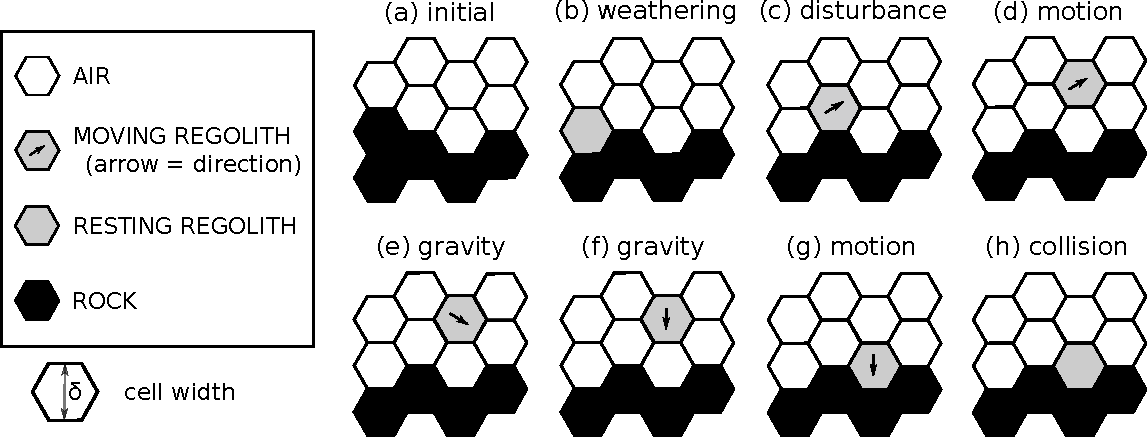
\includegraphics[scale=0.7]{Figures/cell_states_and_transitions.pdf}}
\caption{Illustration of cell states and pairwise transitions in the Grain Facet model. Each cell assigned an integer from 0 to 8 that represents its state (0 is fluid, states 1--6 represent the six directions of motion, state 7 is resting sediment, and state 8 is rock). (Figure modified from \citet{tucker2018lattice}).}
\label{fig:cellstates}
\end{figure}

\begin{figure}[ht!]
\centerline{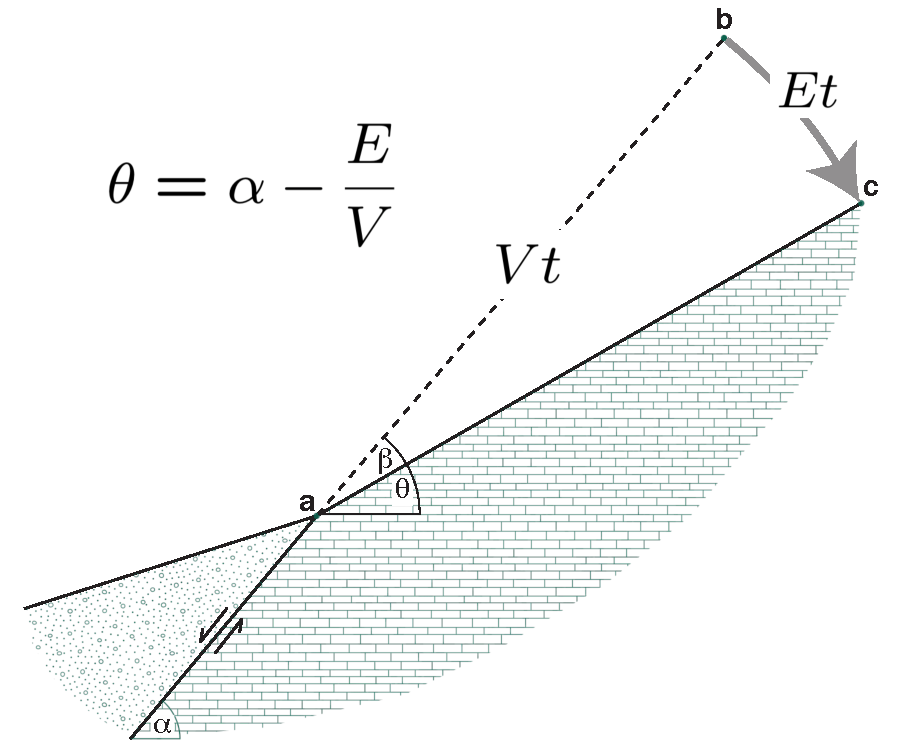
\includegraphics{Figures/facet_schematic.pdf}}
\caption{}
\label{fig:facetschem}
\end{figure}

\begin{figure}[ht!]
\centerline{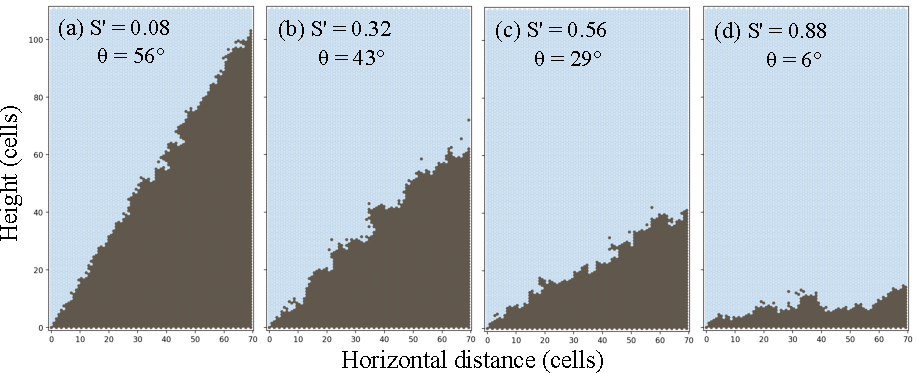
\includegraphics{Figures/dissolution_model_profiles.pdf}}
\caption{Simulated facet cross-sectional profiles formed under a combination of fault slip and dissolution. Dark gray indicates rock, and light blue is air. Labels show the dimensionless effective dissolution efficiency, $S'$ (equation~\ref{eq:nddissefficiency}), and the average facet slope angle, $\gamma$.}
\label{fig:dissruns}
\end{figure}

\begin{figure}[ht!]
\centerline{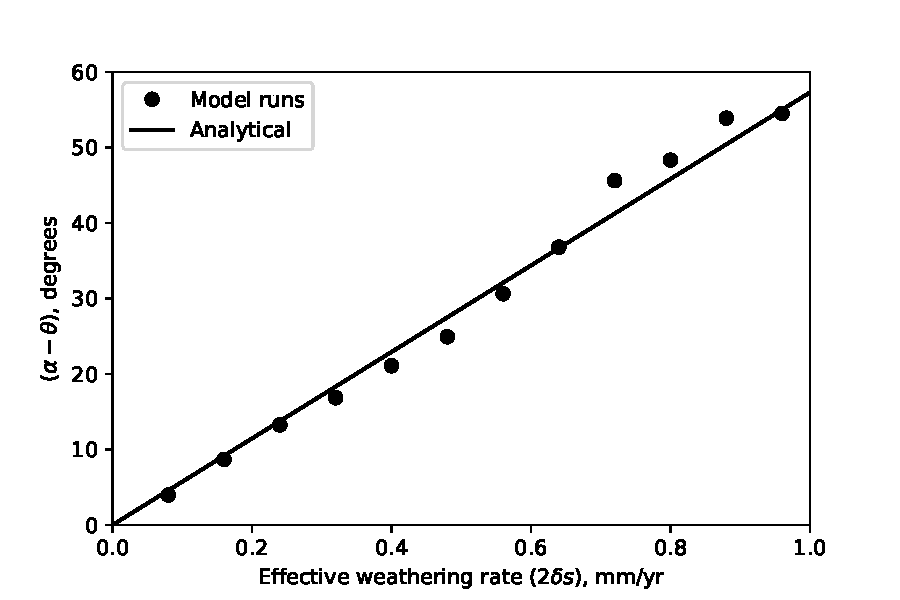
\includegraphics{Figures/angle_vs_dissolution.pdf}}
\caption{Difference in angle between fault plane ($\alpha$) and facet ($\gamma$), as a function of the nominal dissolution rate $2\delta s$, from runs with fault slip and dissolution (only). Solid circles show individual model runs, and line shows the prediction of equation~\ref{eq:angdif}.}
\label{fig:angdiss}
\end{figure}

\begin{figure}[ht!]
\centerline{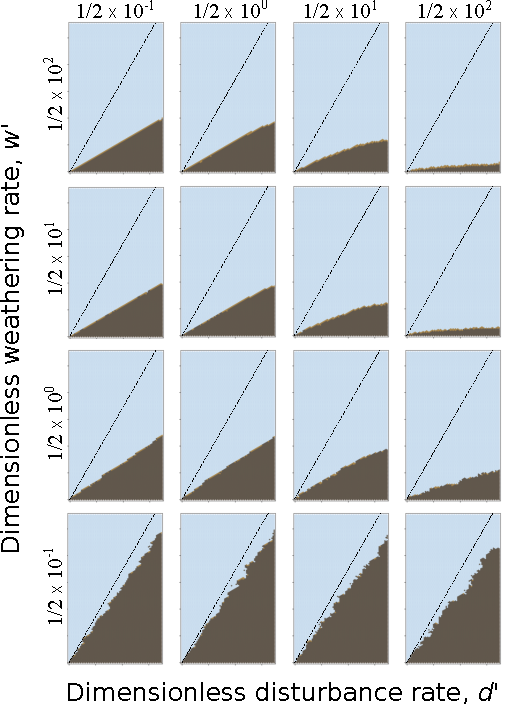
\includegraphics{Figures/four_by_four_profiles_in_d-w_space.pdf}}
\caption{Examples of simulated facet profiles at varying values of $d'$ and $w'$. Dotted line shows projected fault plane.}
\label{fig:dwprofiles}
\end{figure}

\begin{figure}[ht!]
\centerline{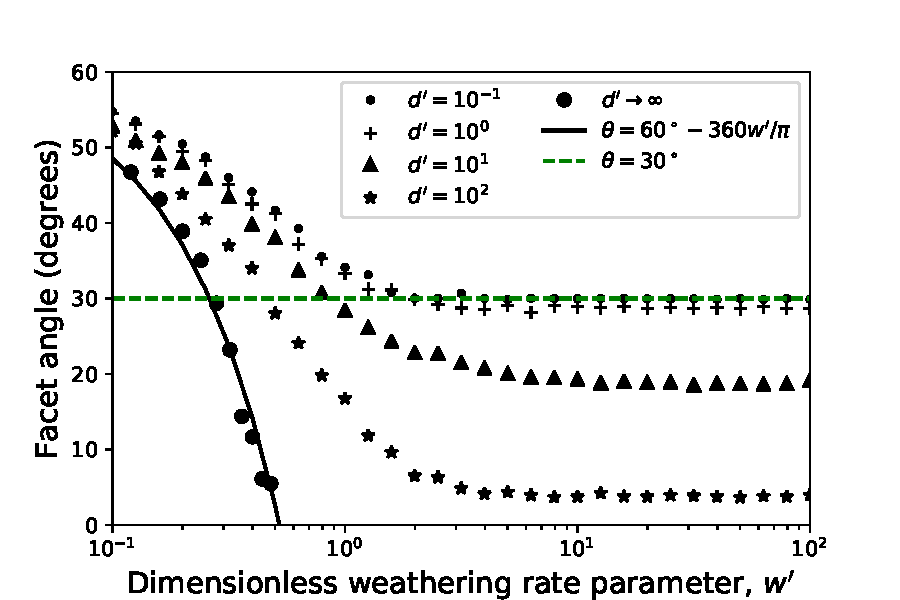
\includegraphics{Figures/facet_angle_vs_wprime.pdf}}
\caption{Modeled equilibrium facet angle as a function of weathering and disturbance rate parameters. Solid line shows the analytical solution for the case in which no regolith is produced (all rock dissolves), which corresponds to an effectively infinite disturbance rate. Dashed line shows the model's 30$^\circ$ effective angle of repose.}
\label{fig:angw}
\end{figure}

\begin{figure}[ht!]
\centerline{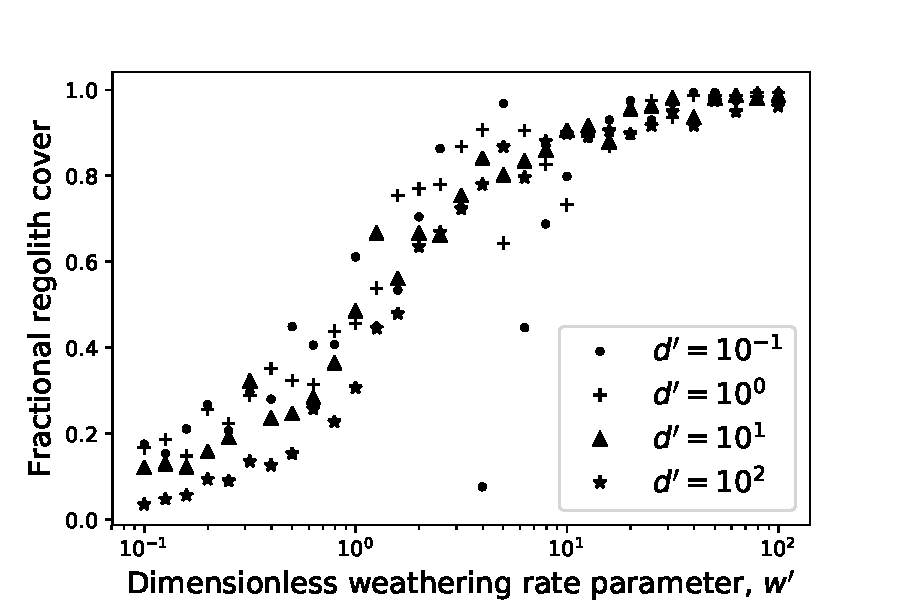
\includegraphics{Figures/reg_cover_vs_wprime.pdf}}
\caption{Modeled regolith cover proportion for steady facets, as a function of weathering and disturbance rate parameters. Scatter around the sigmoidal curve reflects stochastic variability.}
\label{fig:regw}
\end{figure}

\begin{figure}[ht!]
\centerline{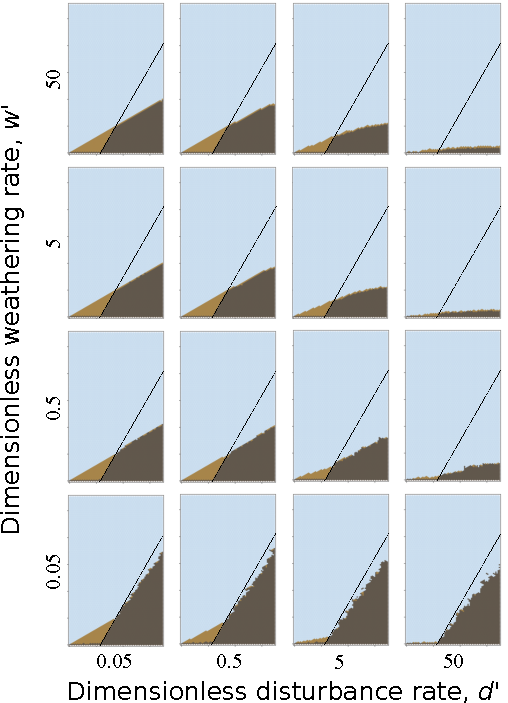
\includegraphics{Figures/four_by_four_profiles_colluvial_wedge.pdf}}
\caption{Simulated facet profiles showing the development of a colluvial wedge on the hangingwall.}
\label{fig:colluv}
\end{figure}

\begin{figure}[ht!]
\centerline{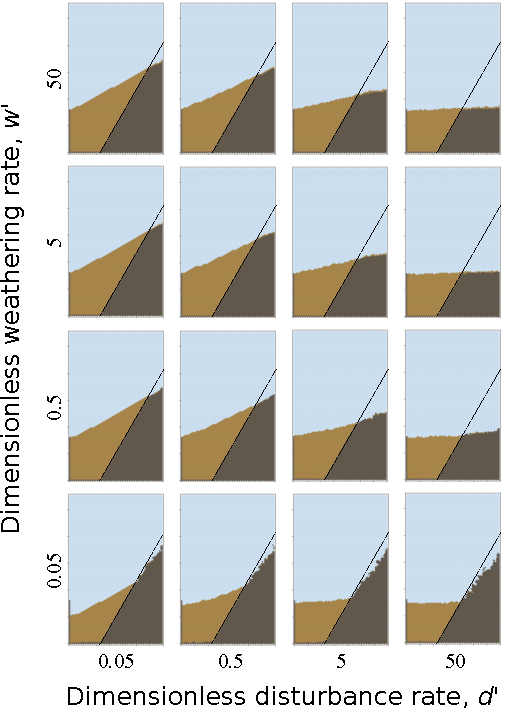
\includegraphics{Figures/four_by_four_profiles_baselevel_rise.pdf}}
\caption{Simulated facet profiles with a rising baselevel along the left model boundary, representing an aggrading hangingwall basin.}
\label{fig:baselevelrise}
\end{figure}









%% ------------------------------------------------------------------------ %%





%%% End of body of article

%%%%%%%%%%%%%%%%%%%%%%%%%%%%%%%%
%% Optional Appendix goes here
%
% \appendix resets counters and redefines section heads
% but doesn't print anything.
% After typing \appendix
%
%\section{Here Is Appendix Title}
% will show
% A: Here Is Appendix Title
%

%%%%%%%%%%%%%%%%%%%%%%%%%%%%%%%%%%%%%%%%%%%%%%%%%%%%%%%%%%%%%%%%
%
% Optional Glossary, Notation or Acronym section goes here:
%
%%%%%%%%%%%%%%
% Glossary is only allowed in Reviews of Geophysics


%
%%%%%%%%%%%%%%
% Acronyms
 

%
%%%%%%%%%%%%%%
% Notation




%%%%%%%%%%%%%%%%%%%%%%%%%%%%%%%%%%%%%%%%%%%%%%%%%%%%%%%%%%%%%%%%
%
%  ACKNOWLEDGMENTS

\acknowledgments
thanks




%%  REFERENCE LIST AND TEXT CITATIONS
%
% Either type in your references using
%
% \begin{thebibliography}{}
% \bibitem{}
% Text
% \end{thebibliography}
%
% Or, to use BibTeX:
%
% Follow these steps
%
% 1. Type in \bibliography{<name of your .bib file>}
%    Run LaTeX on your LaTeX file.
%
% 2. Run BiBTeX on your LaTeX file.
%
% 3. Open the new .bbl file containing the reference list and
%   copy all the contents into your LaTeX file here.
%
% 4. Run LaTeX on your new file which will produce the citations.
%
% AGU does not want a .bib or a .bbl file. Please copy in the contents of your .bbl file here.



%\bibliography{gt_library.bib}

\begin{thebibliography}{1}
\providecommand{\natexlab}[1]{#1}
\expandafter\ifx\csname urlstyle\endcsname\relax
  \providecommand{\doi}[1]{doi:\discretionary{}{}{}#1}\else
  \providecommand{\doi}{doi:\discretionary{}{}{}\begingroup
  \urlstyle{rm}\Url}\fi

\bibitem[{\textit{Boulton and Whittaker}(2009)}]{boulton2009quantifying}
Boulton, S., and A.~Whittaker (2009), Quantifying the slip rates, spatial
  distribution and evolution of active normal faults from geomorphic analysis:
  Field examples from an oblique-extensional graben, southern turkey,
  \textit{Geomorphology}, \textit{104}(3-4), 299--316.

\bibitem[{\textit{Tucker et~al.}(2018)\textit{Tucker, McCoy, and
  Hobley}}]{tucker2018lattice}
Tucker, G.~E., S.~W. McCoy, and D.~E. Hobley (2018), A lattice grain model of
  hillslope evolution, \textit{Earth Surface Dynamics}, \textit{6}(3),
  563--582.


\end{thebibliography}





%%%%%%%%%%%%%%%%%%%%%%%%%%%%%%%%%%%%%%%%%
% Track Changes:
% To add words, \added{<word added>}
% To delete words, \deleted{<word deleted>}
% To replace words, \replace{<word to be replaced>}{<replacement word>}

% At the end of the document, use \listofchanges, which will list the
% changes and the page and line number where the change was made.

% When final version, \listofchanges will not produce anything,
% \added{} word will be printed, \deleted{} will take away the word,
% \replaced{}{} will print only the 2nd argument.

%%%
%\listofchanges
%%%

\end{document}

%%%%%%%%%%%%%%%%%%%%%%%%%%%%%%%%%%%%%
%% Supporting Information
%% (Optional) See AGUSuppInfoSamp.tex/pdf for requirements
%% for Supporting Information.
%%%%%%%%%%%%%%%%%%%%%%%%%%%%%%%%%%%%%


%%%%%%%%%%%%%%%%%%%%%%%%%%%%%%%%%%%%%%%%%%%%%%%%%%%%%%%%%%%%%%%

%More Information and Advice:

%% ------------------------------------------------------------------------ %%
%
%  SECTION HEADS
%
%% ------------------------------------------------------------------------ %%

% Capitalize the first letter of each word (except for
% prepositions, conjunctions, and articles that are
% three or fewer letters).

% AGU follows standard outline style; therefore, there cannot be a section 1 without
% a section 2, or a section 2.3.1 without a section 2.3.2.
% Please make sure your section numbers are balanced.
% ---------------
% Level 1 head
%
% Use the \section{} command to identify level 1 heads;
% type the appropriate head wording between the curly
% brackets, as shown below.
%
%An example:
%\section{Level 1 Head: Introduction}
%
% ---------------
% Level 2 head
%
% Use the \subsection{} command to identify level 2 heads.
%An example:
%\subsection{Level 2 Head}
%
% ---------------
% Level 3 head
%
% Use the \subsubsection{} command to identify level 3 heads
%An example:
%\subsubsection{Level 3 Head}
%
%---------------
% Level 4 head
%
% Use the \subsubsubsection{} command to identify level 3 heads
% An example:
%\subsubsubsection{Level 4 Head} An example.
%
%% ------------------------------------------------------------------------ %%
%
%  IN-TEXT LISTS
%
%% ------------------------------------------------------------------------ %%
%
% Do not use bulleted lists; enumerated lists are okay.
% \begin{enumerate}
% \item
% \item
% \item
% \end{enumerate}
%
%% ------------------------------------------------------------------------ %%
%
%  EQUATIONS
%
%% ------------------------------------------------------------------------ %%

% Single-line equations are centered.
% Equation arrays will appear left-aligned.

% To create multiline equations, use the
% \begin{eqnarray} and \end{eqnarray} environment
% as demonstrated below.
%\begin{eqnarray}
%  x_{1} & = & (x - x_{0}) \cos \Theta \nonumber \\
%        && + (y - y_{0}) \sin \Theta  \nonumber \\
%  y_{1} & = & -(x - x_{0}) \sin \Theta \nonumber \\
%        && + (y - y_{0}) \cos \Theta.
%\end{eqnarray}

%If you don't want an equation number, use the star form:
%\begin{eqnarray*}...\end{eqnarray*}

% Break each line at a sign of operation
% (+, -, etc.) if possible, with the sign of operation
% on the new line.

% Indent second and subsequent lines to align with
% the first character following the equal sign on the
% first line.

% Use an \hspace{} command to insert horizontal space
% into your equation if necessary. Place an appropriate
% unit of measure between the curly braces, e.g.
% \hspace{1in}; you may have to experiment to achieve
% the correct amount of space.


%% ------------------------------------------------------------------------ %%
%
%  EQUATION NUMBERING: COUNTER
%
%% ------------------------------------------------------------------------ %%

% You may change equation numbering by resetting
% the equation counter or by explicitly numbering
% an equation.

% To explicitly number an equation, type \eqnum{}
% (with the desired number between the brackets)
% after the \begin{equation} or \begin{eqnarray}
% command.  The \eqnum{} command will affect only
% the equation it appears with; LaTeX will number
% any equations appearing later in the manuscript
% according to the equation counter.
%

% If you have a multiline equation that needs only
% one equation number, use a \nonumber command in
% front of the double backslashes (\\) as shown in
% the multiline equation above.

% If you are using line numbers, remember to surround
% equations with \begin{linenomath*}...\end{linenomath*}

%  To add line numbers to lines in equations:
%  \begin{linenomath*}
%  \begin{equation}
%  \end{equation}
%  \end{linenomath*}



